\chapter{Implementation}

\section{Programming Language Selection}

The decision to utilize Python as the primary development language stemmed from the specific demands of deep learning and computer vision tasks. Python provides an extensive and mature ecosystem, notably featuring frameworks which are critical for the neural network components of the proposed system. Its flexibility allowed for rapid prototyping of the multi-object tracking pipeline while maintaining enough performance, when paired with compiled libraries, to handle live video ingestion. The integration of various specialized libraries—ranging from mathematical computation to graphical map rendering—was significantly streamlined by Python's package management and interoperability.

\section{Platform Selection}

Executing complex visual detection alongside trajectory forecasting in real-time requires substantial computational bandwidth. The development and deployment were carried out on environments equipped with NVIDIA graphical processing units, leveraging the CUDA parallel computing platform. This hardware acceleration was strictly necessary because standard CPU execution would incur severe latency during the frame-by-frame inference stages. Developing on both Windows and Linux environments ensured that the final surveillance pipeline remained adaptable and not rigidly bound to a single operating system, thereby facilitating easier deployment in varying maritime control centers.

\section{Code Conventions}

Maintaining consistency across the codebase was prioritized to facilitate debugging and future scalability. The implementation adhered closely to the PEP 8 style guidelines, standardizing naming conventions, indentation, and structural modularity throughout the project scripts. Adopting these established practices ensures that the logic governing trajectory prediction and sensor fusion remains accessible to subsequent researchers or engineers who might inherit the system, thereby reducing the friction typically associated with understanding complex, multi-stage pipelines.

\section{Difficulties Encountered and Strategies Used to Tackle}

Several distinct challenges emerged during the integration of visual tracking with geospatial data. A prominent issue involved frequent visual occlusions and severe glare from the water surface, which caused the baseline tracker to frequently drop ship identities. To mitigate this, the architecture incorporated DeepOCSORT backed by an OSNet appearance-based re-identification network, allowing the system to recover tracking IDs based on ship features rather than relying purely on spatial overlap. Another significant hurdle was aligning the asynchronous AIS telemetry with the continuous camera feed. This discrepancy was resolved by employing a Kalman filter, which effectively smoothed the noisy camera projections while correcting the position updates using the sparse AIS reports.

\section{Data Set Description}

Training robust models for maritime environments demands diverse and representative data. Rather than relying on a single static repository, the foundational data was curated by sampling numerous maritime video feeds under varying environmental conditions. This included variations in sea states, varying times of the day, and different vessel densities. The collected frames underwent manual verification to ensure bounding box accuracy, which proved vital for fine-tuning the YOLOv8 detector. Detailed specifications regarding dataset volume and partition ratios are expanded upon during the subsequent evaluation setup.

\section{System Architecture and Algorithms Used}

At the highest level, the implementation is structured around a sequential pipeline architecture. Each functional stage operates with a degree of independence but communicates with the next via strictly defined data interfaces. Decoupling the modules in this manner is a deliberate design choice to prevent computational bottlenecks—such as the heavy processing required during sequence prediction—from stalling the continuous ingestion of the live video feed. 

The overall framework is compartmentalized into six interconnected stages: continuous video ingestion, frame-level ship detection, persistent multi-object tracking, sensor fusion, recurrent trajectory prediction, and final geospatial visualization. Organizing the system into these discrete steps ensures that data transitions smoothly from raw pixel arrays all the way to actionable geographic intelligence. Figure~\ref{fig:deployment} provides a detailed schematic of how these disparate modules are deployed and traces the flow of information across the backend environment.

\begin{figure}[H]
\centering
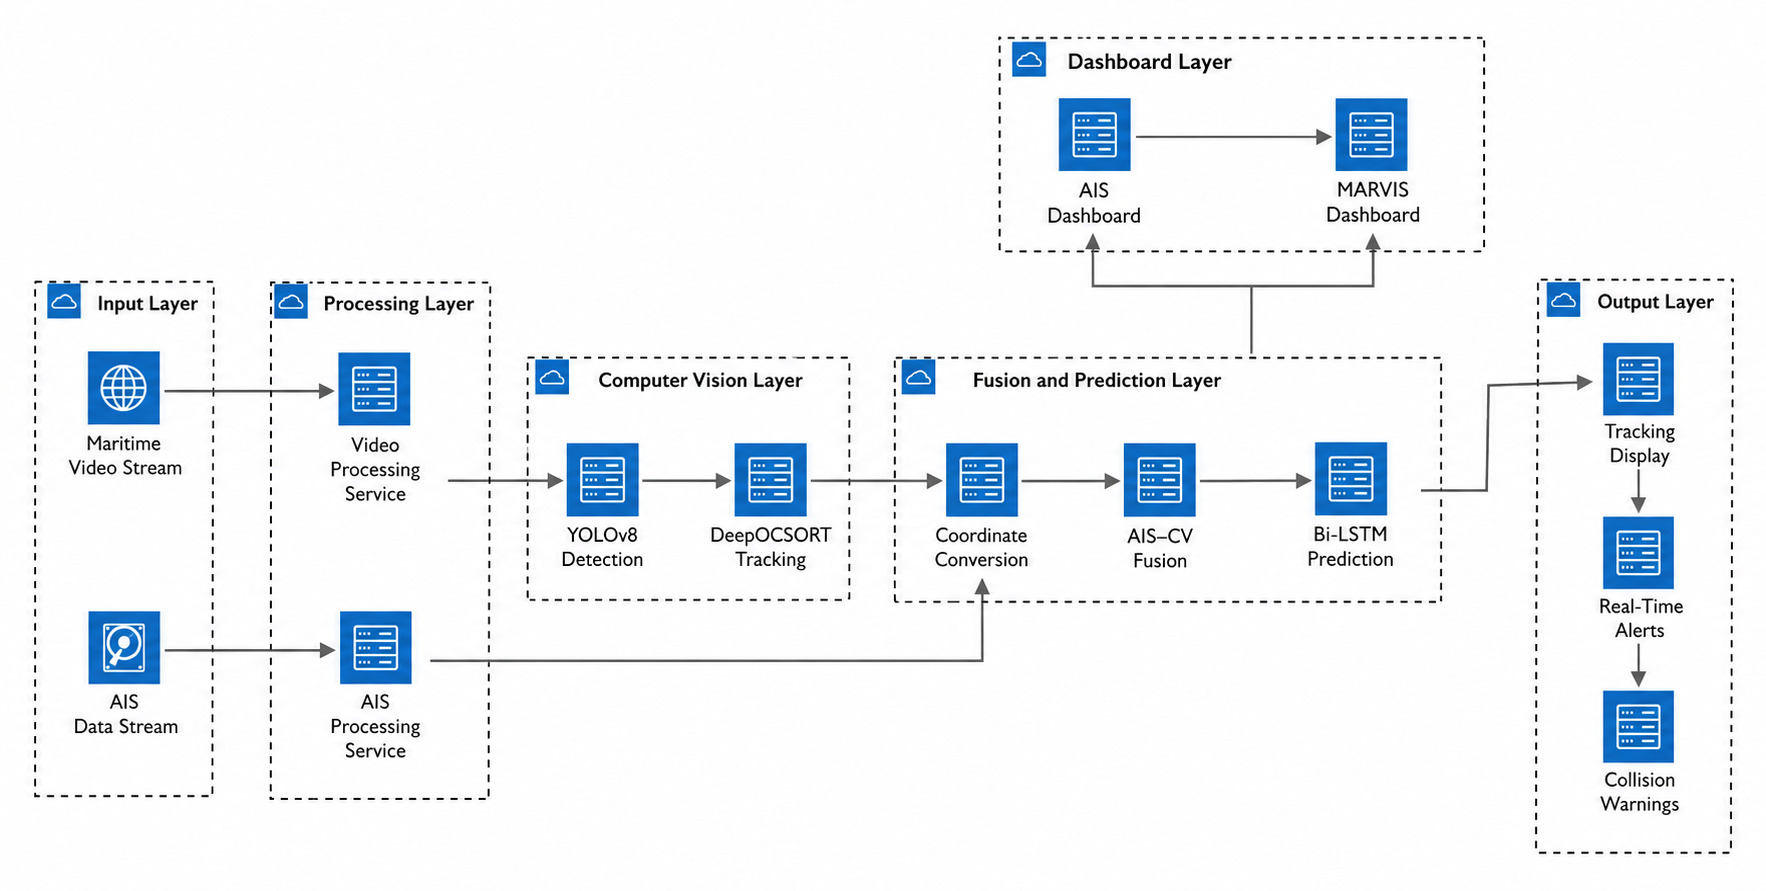
\includegraphics[width=0.95\textwidth]{Chapter4/Figures/deployment_architecture.jpeg}
\caption{Deployment and Backend Communication Architecture of Proposed Maritime Surveillance System}
\label{fig:deployment}
\end{figure}

\subsection{Development Environment Configuration}

Constructing the software stack involved selecting tools that could manage high-throughput data streams while providing robust mathematical primitives. The central logic relies on Python 3.8, a decision heavily influenced by its dominant position in the artificial intelligence sector. All deep learning operations, in particular the execution of the \gls{yolov8} detection weights and the forward passes of the \gls{lstm} trajectory network, were built upon the \gls{pytorch} framework. This allowed for precise control over tensor operations and memory management during model inference.

Handling the visual aspects of the system required a highly optimized library capable of raw image manipulation. \gls{opencv} was tasked with managing the video ingestion pipeline, executing the frame-by-frame extraction process, and overlaying the graphical bounding boxes directly onto the live visual output. Operating silently behind the scenes, numerical and tabular data management was delegated to NumPy and Pandas. These libraries efficiently handled the dynamic arrays that store the coordinate history of ship centroids, as well as the sliding sequence buffers essential for the recurrent neural network. The visualization duties were distinctly divided based on their application: Matplotlib served as the primary tool for generating static analytical plots during development, whereas Folium was integrated to construct the interactive, real-time geographical maps presented to the end user.

Hardware capabilities dictated much of the deployment strategy. The entire surveillance pipeline was configured to run on an \gls{nvidia} \gls{gpu}-enabled machine, leaning heavily on \gls{cuda} acceleration to process matrix multiplications. Attempting to execute concurrent deep learning tasks—such as bounding box detection, appearance-based re-identification, and sequential coordinate forecasting—on a standard CPU at thirty frames per second would result in immediate thermal throttling and unacceptable processing delays. The iterative process of writing the logic, troubleshooting errors, and testing algorithmic variations was primarily facilitated through Visual Studio Code and Jupyter Notebook environments.

\subsection{Data Preparation and Model Training}

The effectiveness of the vision models within the real-time pipeline depended heavily on the quality of their initial training. The raw maritime video footage was systematically parsed into discrete frames at a predetermined sampling interval. This approach generated a comprehensive dataset capable of representing a wide array of sea states, fluctuating lighting situations, and complex scenarios involving vessel occlusion. Every extracted frame was carefully annotated, utilizing the standard \gls{yolo} bounding box format to log the object class identifier alongside the normalized center coordinates, width, and height for each target.

A rigorous partitioning strategy was enforced to guard against model overfitting. The compiled dataset was divided into training, validation, and testing segments according to a 70:20:10 distribution. As the models cycled through the training phase, a suite of dynamic augmentation techniques was introduced to artificially expand the variance of the data. Transformations such as horizontal flipping, mosaic assembling, random spatial cropping, and unpredictable brightness adjustments compelled the neural network to develop generalized features rather than memorizing the training images, a critical factor for performing in chaotic maritime settings.

Focusing on the detection architecture, the \gls{yolov8} model was not trained from scratch. It was initialized using weights pretrained on the extensive COCO dataset, and then subjected to targeted fine-tuning using transfer learning techniques. The optimization process relied on Stochastic Gradient Descent (SGD) paired with a Cosine Annealing scheduler to smoothly adjust the learning rate. An early stopping mechanism continuously monitored the mean Average Precision (mAP) against the validation partition, automatically halting the training cycles the moment performance gains plateaued. During live operations, the trained model is subjected to strict inference constraints. It enforces a minimum confidence threshold of 0.5 and a non-maximum suppression (\gls{nms}) intersection over union (\gls{iou}) threshold of 0.45. By discarding predictions that fall short of this confidence bar, the system prevents the subsequent tracking logic from becoming saturated with erroneous vessel detections.

Once a set of bounding boxes is confirmed, the data is handed over to the \gls{deepocsort} multi-object tracker. The tracking parameters were carefully tuned, dictating a maximum track age of thirty frames before an unseen object is forgotten, and requiring a minimum of three consecutive visual hits to formally establish a new target track. To tackle the difficult problem of identity preservation, particularly when ships momentarily disappear from view, \gls{deepocsort} leans on an \gls{osnet} feature extractor. This sub-network generates a dense, compact visual embedding unique to each ship's appearance. In practice, the system first tries to link incoming detections to established tracks by evaluating spatial overlap. Should this spatial matching fail—a common occurrence when boats obscure one another—the system pivots to comparing the generated \gls{osnet} embeddings via cosine similarity. This appearance-based fallback often successfully re-identifies the vessel. The confirmed spatial coordinates are then appended to an ongoing buffer, setting the stage for subsequent motion calculations.

\subsection{Motion Estimation and Sensor Fusion}

The continuous buffering of centroid coordinates for every confirmed track forms the basis for extracting granular motion parameters between consecutive frames. The instantaneous speed of a vessel is calculated by measuring the Euclidean distance its bounding box center travels across the camera sensor, scaled by the time interval. Simultaneously, the heading is deduced by analyzing the horizontal and vertical shift patterns utilizing fundamental trigonometric functions. To make this information immediately digestible for a human operator, the raw angular calculations are translated into standardized cardinal and intermediate compass directions before being actively drawn onto the surveillance monitor.

Operating alongside the vision pipeline, the sensor fusion component is responsible for processing the incoming stream of \gls{ais} broadcast telemetry. These maritime transmissions contain highly reliable metadata, including the unique \gls{mmsi} identifier, exact global coordinates, speed over ground (\gls{sog}), and course over ground (\gls{cog}). The primary challenge lies in combining the pixel-space tracking data with this geographic telemetry. To bridge this gap, the system applies a homographic transformation matrix, mathematically projecting the pixel coordinates onto a geographic plane. Following this transformation, a nearest-neighbor algorithm evaluates the Haversine distance separating the projected camera positions and the corresponding \gls{ais} reports to establish a definitive link between the two sources.

Upon successful data association, the rich \gls{ais} metadata is grafted onto the ongoing visual track. It is understood, however, that visual projections derived from a camera feed possess an inherent degree of noise and jitter. To counter this instability, a Kalman filtering mechanism is introduced into the fused data state. The filter effectively balances the rapid, high-frequency updates provided by the optical tracker against the less frequent but highly precise \gls{ais} positional reports. The result of this filtering process is a remarkably stable, real-time approximation of the target's true geographic location and movement vector, an operation visualized in Figure~\ref{fig:fusion}.

\begin{figure}[H]
\centering
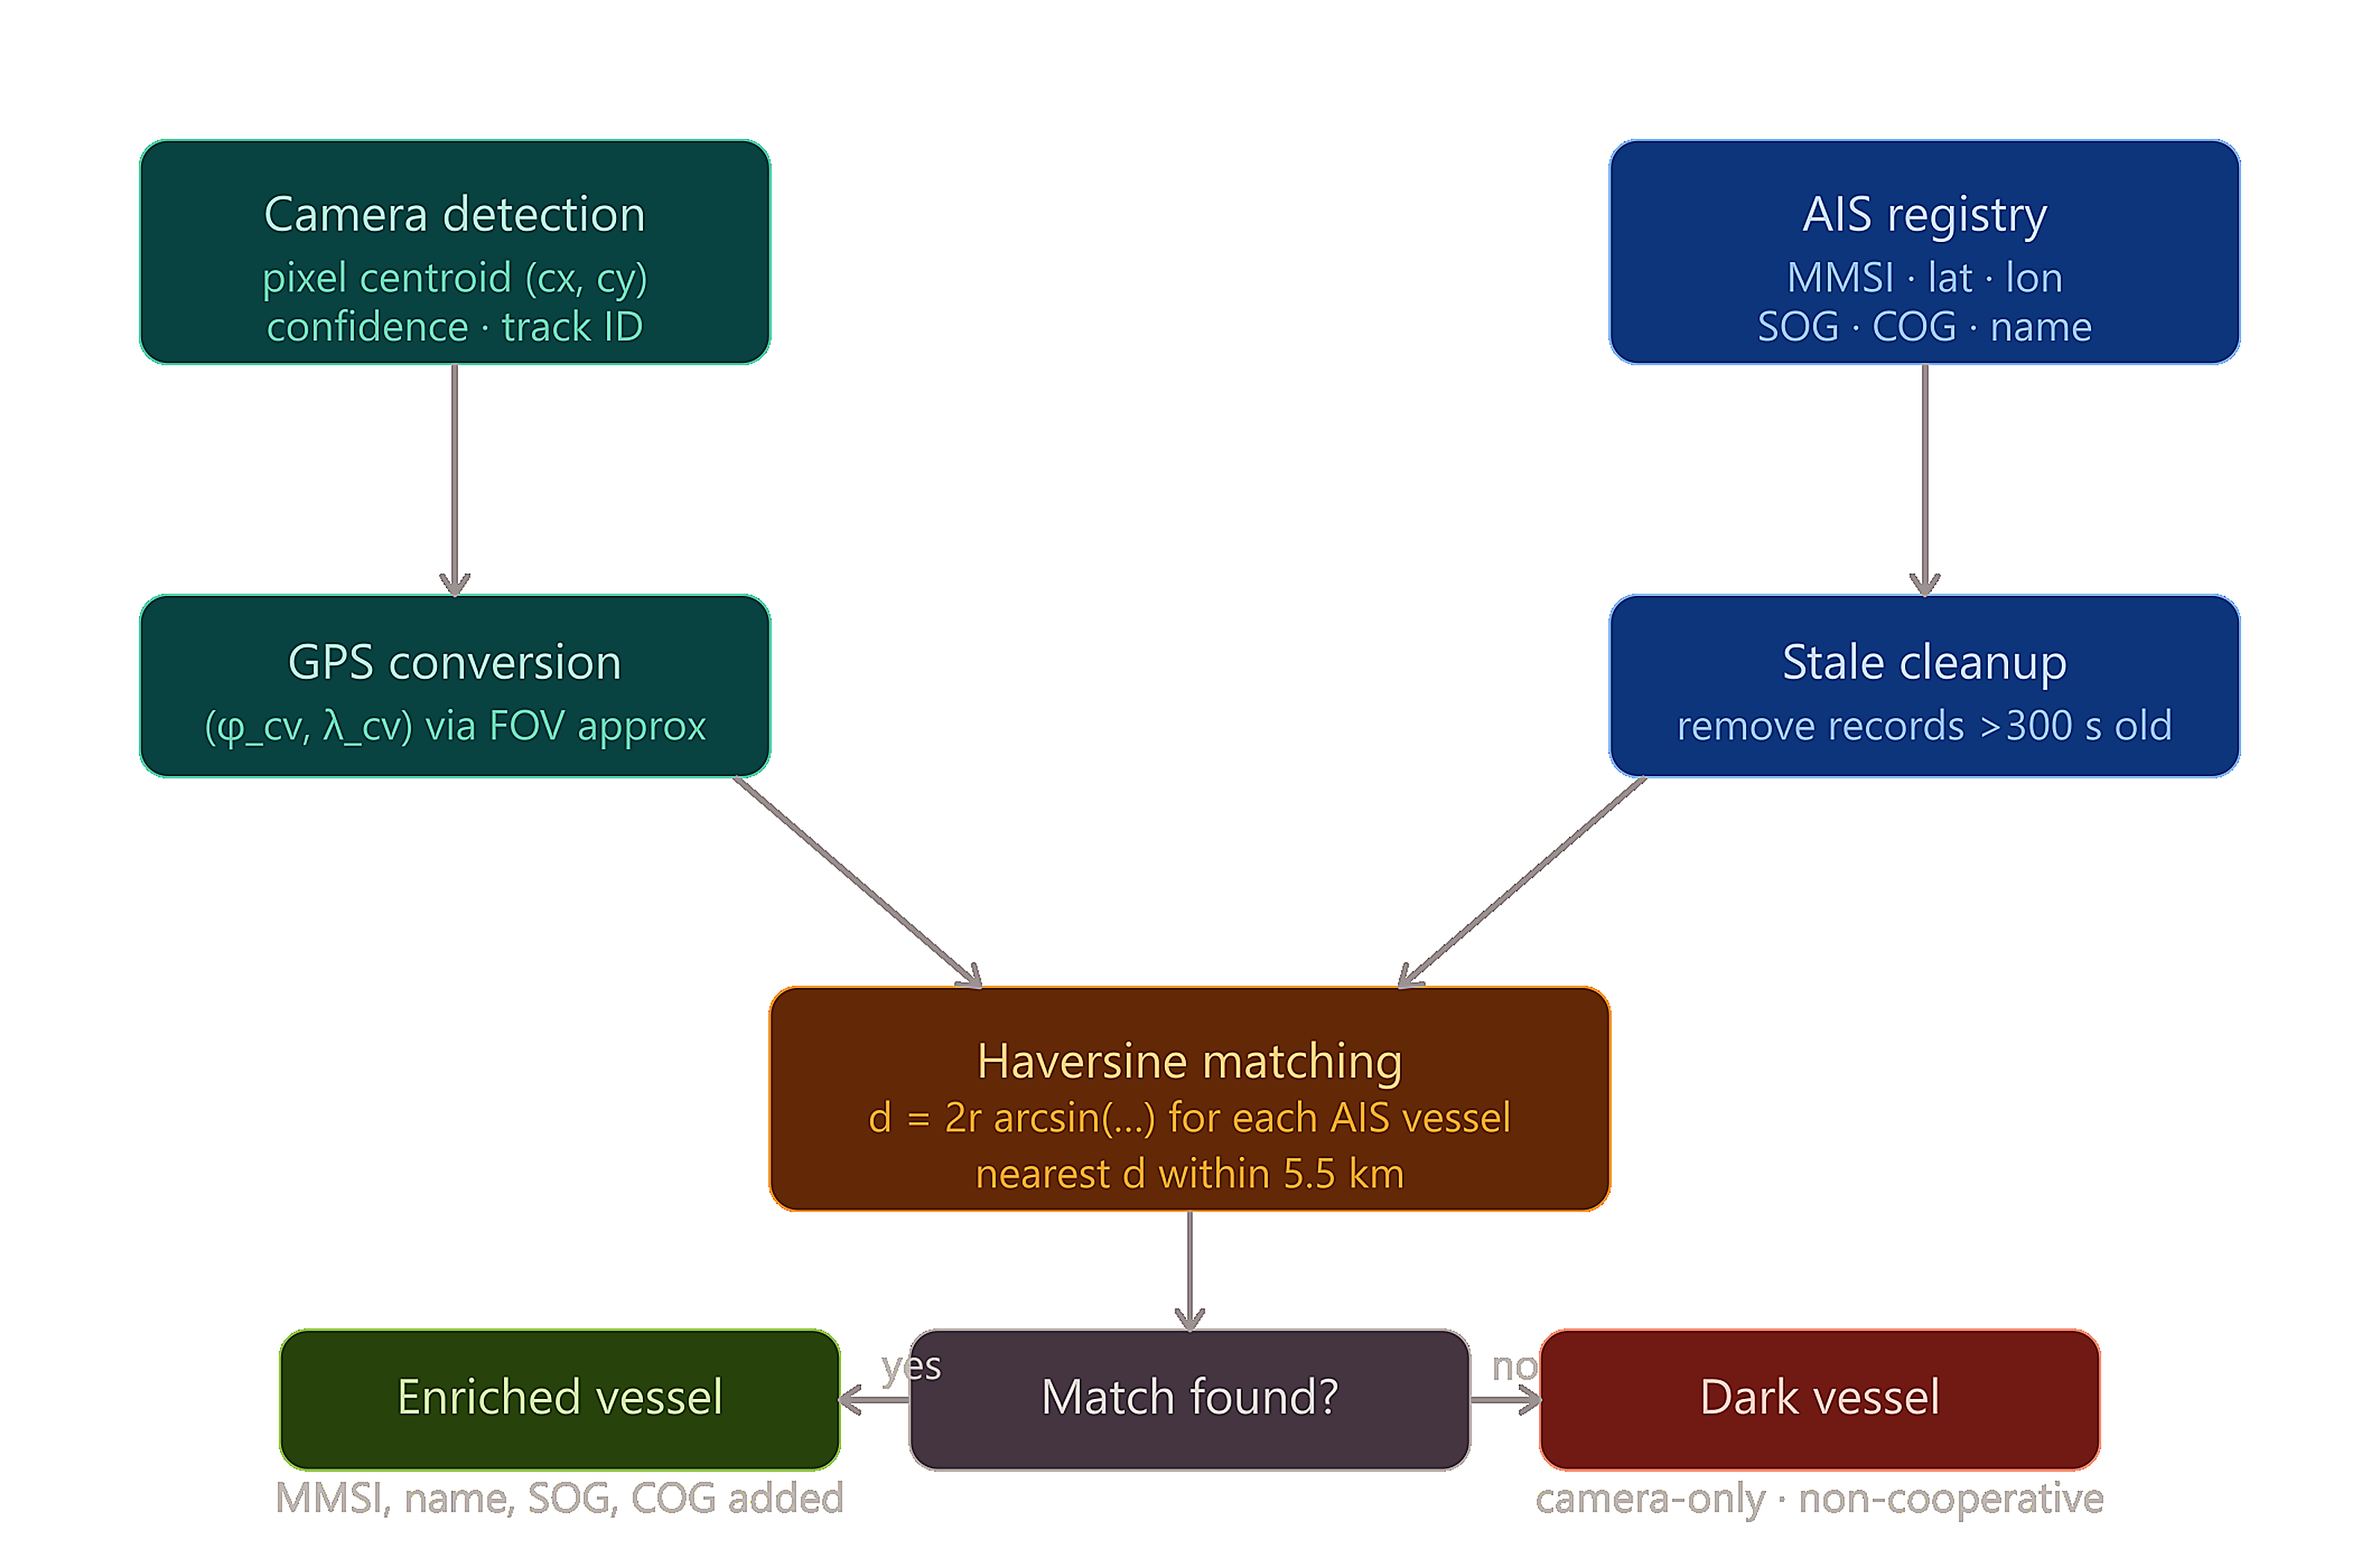
\includegraphics[width=0.95\textwidth]{Chapter4/Figures/cv_ais_fusion.png}
\caption{\gls{ais}--Computer Vision Data Fusion Process}
\label{fig:fusion}
\end{figure}

\subsection{LSTM Trajectory Prediction}

Once a reliable history of geographic positions has been compiled and smoothed by the filter, the data is channeled directly into the trajectory prediction engine. The movement characteristics of large maritime vessels are highly sequential; a ship's future position is inextricably tied to its recent maneuvering behavior. To properly model these deep temporal relationships, a Long Short-Term Memory (\gls{lstm}) neural network architecture was implemented, which significantly outperforms traditional statistical regression techniques when dealing with complex, time-series motion data.

The predictive network is constructed using two stacked \gls{lstm} layers that process the sequential inputs before passing the hidden state into a dense, fully connected output layer to generate the coordinate forecast (Figure~\ref{fig:lstm}). For any given timestep, the input structure consists of a multidimensional feature vector detailing the ship's current latitude and longitude, its measured speed over ground, sine and cosine transformations of its course over ground, alongside a discrete classification label representing the vessel type. Training the network involved feeding it extensive sets of historical movement data, utilizing Mean Squared Error (\gls{mse}) to quantify the loss, and refining the weights using the highly efficient Adam optimization algorithm.

During operational runtime, the system continuously extracts fixed-length temporal slices from the Kalman-filtered location history. These historical windows are pushed through the optimized neural network to map out the vessel's likely path over the coming minutes. A common edge case arises when a ship first enters the camera's field of view, as it lacks the required data history to properly populate the network's input window. To address this without halting the forecasting pipeline, a parallel kinematic linear regression module acts as an immediate fallback mechanism. This ensures that even immature tracks receive a basic trajectory projection while the system accumulates enough historical data points to engage the primary neural network.

\begin{figure}[H]
\centering
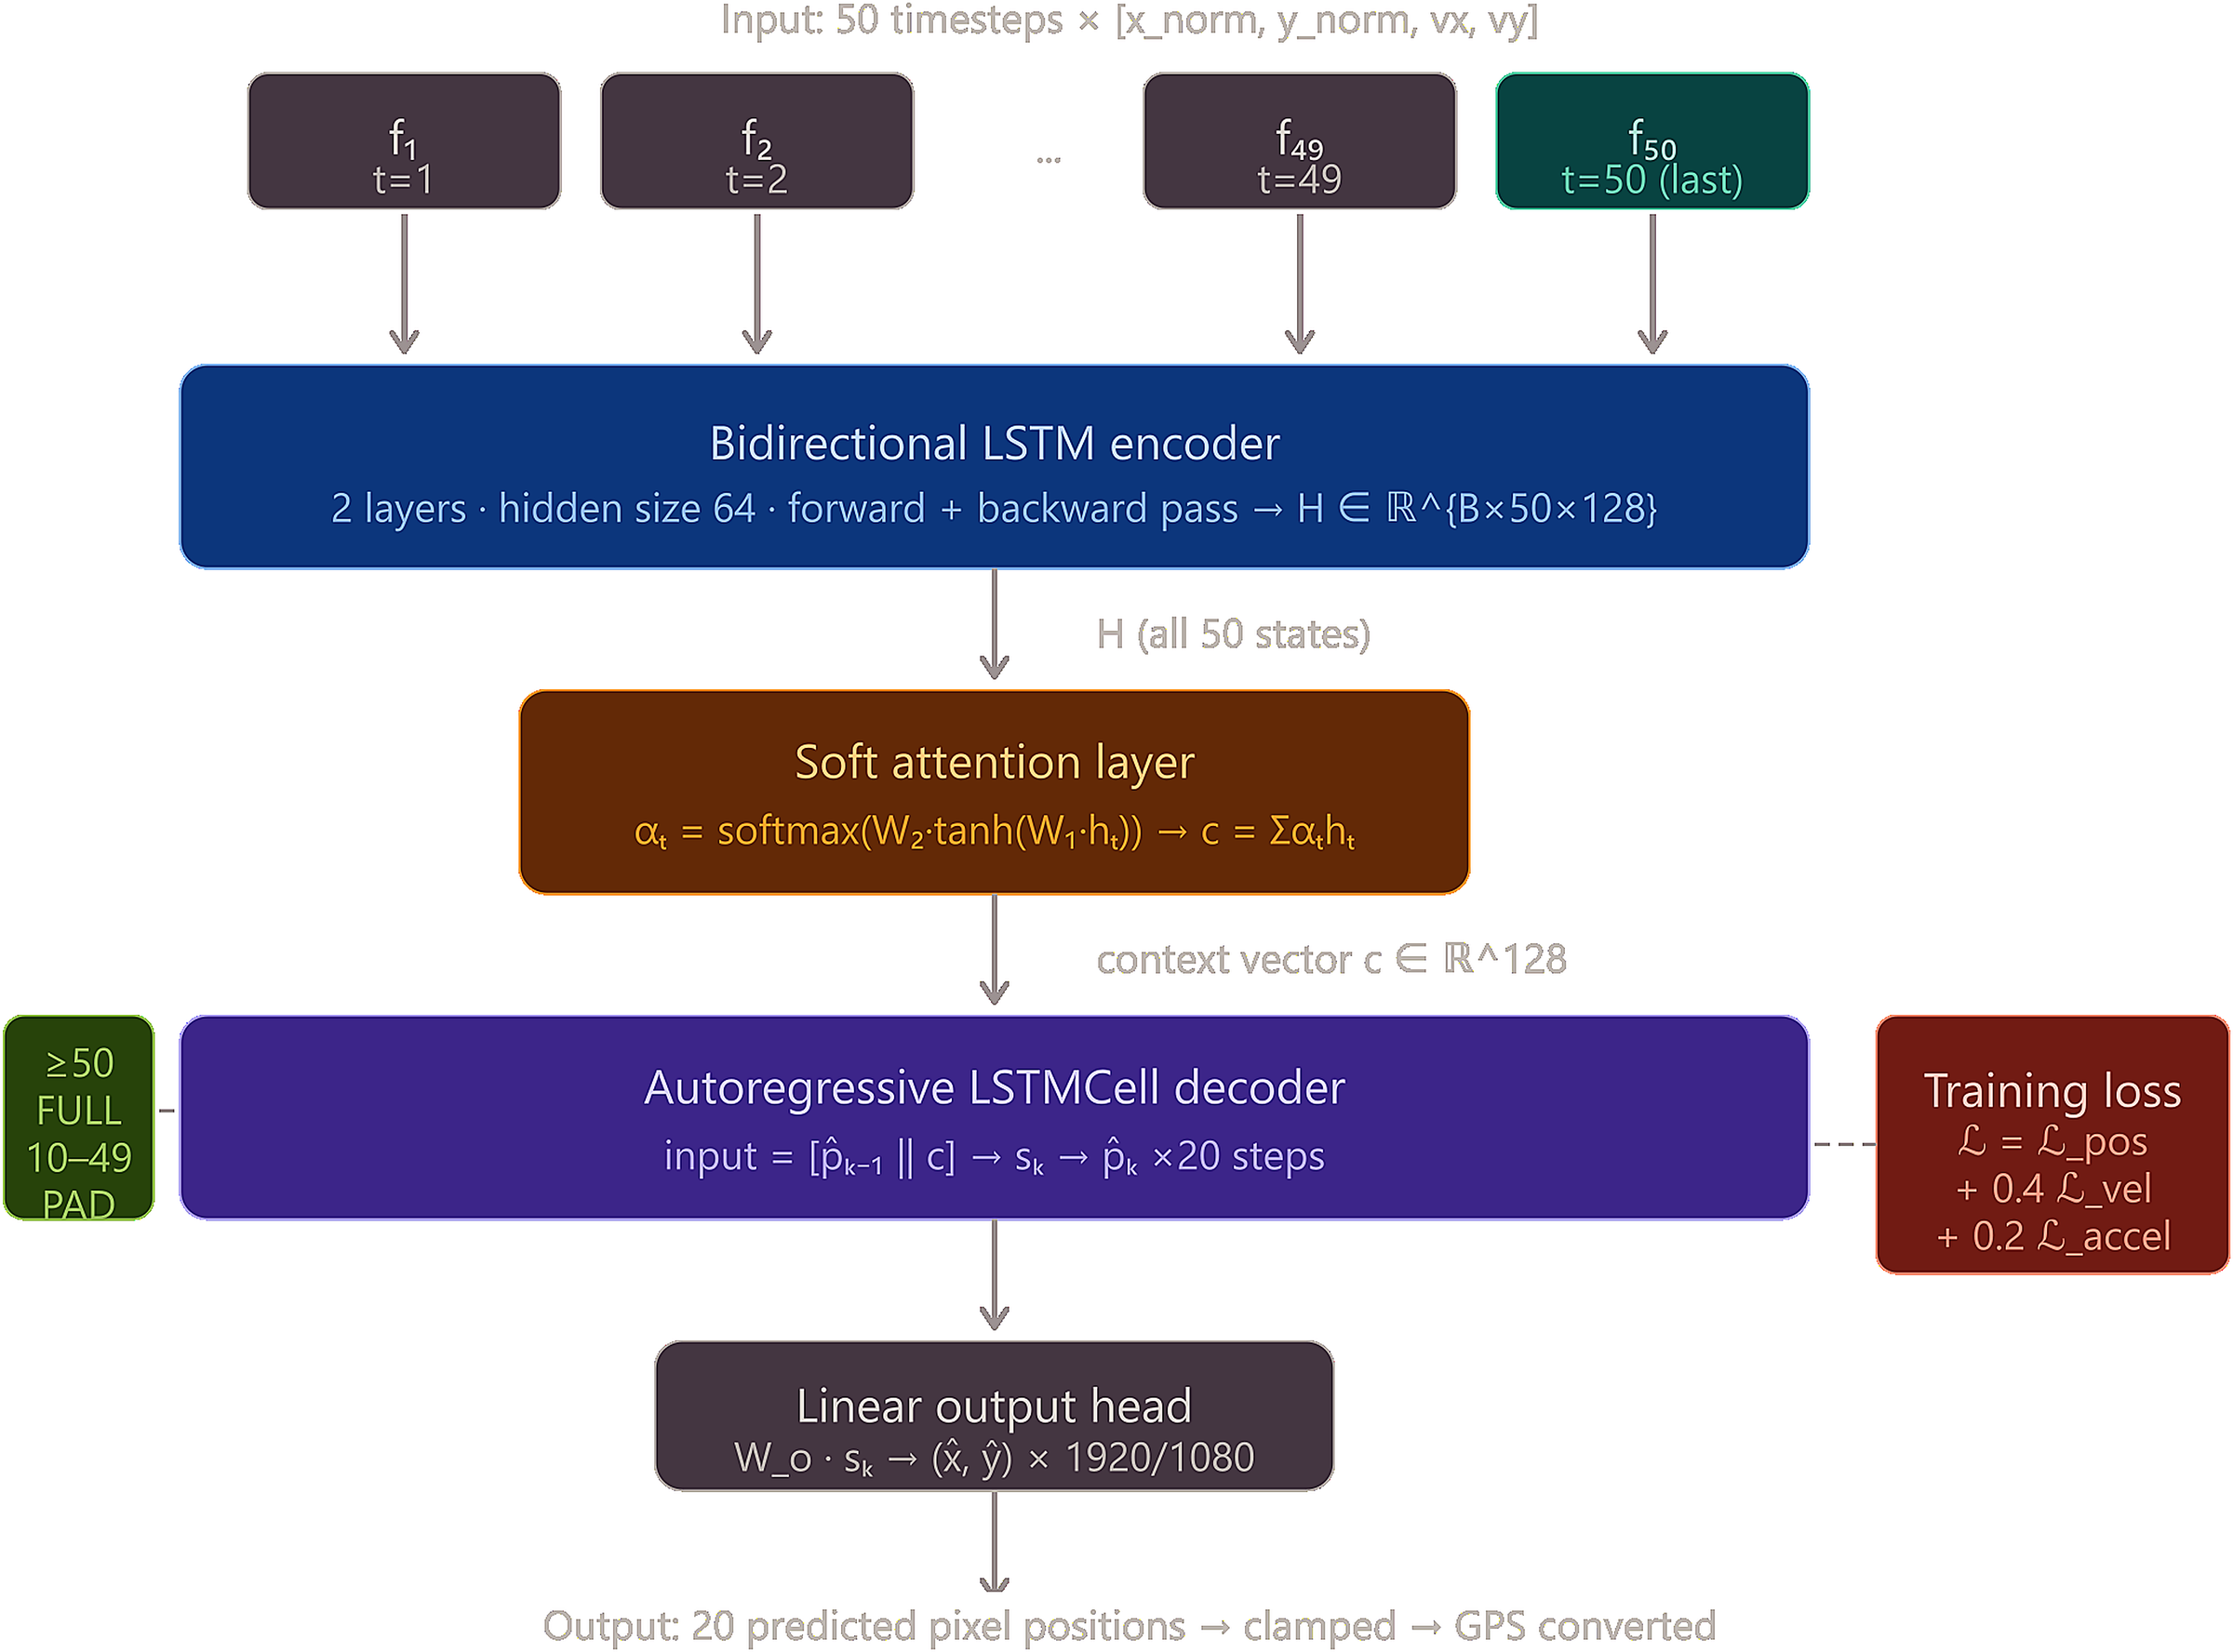
\includegraphics[width=0.90\textwidth]{Chapter4/Figures/lstm_architecture.png}
\caption{\gls{bilstm} Architecture for Vessel Trajectory Prediction}
\label{fig:lstm}
\end{figure}

\subsection{Geospatial Validation and Visualization}

A critical requirement of the system is that all predicted movements align with physical maritime constraints, necessitating a geospatial validation step before any forecasts are displayed to the operator. This post-processing phase routes every predicted coordinate through a stringent land mask filter, comparing the neural network's output against an established topological map detailing landmasses and navigable waters. It is not uncommon for mathematical models to occasionally predict paths that cut across a peninsula during a sharp turning maneuver. When the filter detects such an anomaly, it computationally intervenes, shifting the invalid coordinate to the closest logical body of water. This safeguarding measure strictly enforces environmental realism on all generated predictions.

Following validation, the complete dataset is dispatched to a sophisticated, dual-pronged visualization interface designed for maximum operator awareness. The first output stream leverages \gls{opencv} to draw dynamic bounding boxes, unique identification markers, current speed metrics, and short-term path projections straight over the live camera footage. This provides personnel with immediate, localized visual confirmation of system operations. Simultaneously, the geographic coordinates and long-term trajectory forecasts are transmitted to a web-based dashboard engineered with Folium (Figure~\ref{fig:dashboard}). This secondary interface plots the global locations of all tracked targets on an interactive map, granting operators an expansive, top-down perspective of the entire surveillance sector.

\begin{figure}[H]
\centering
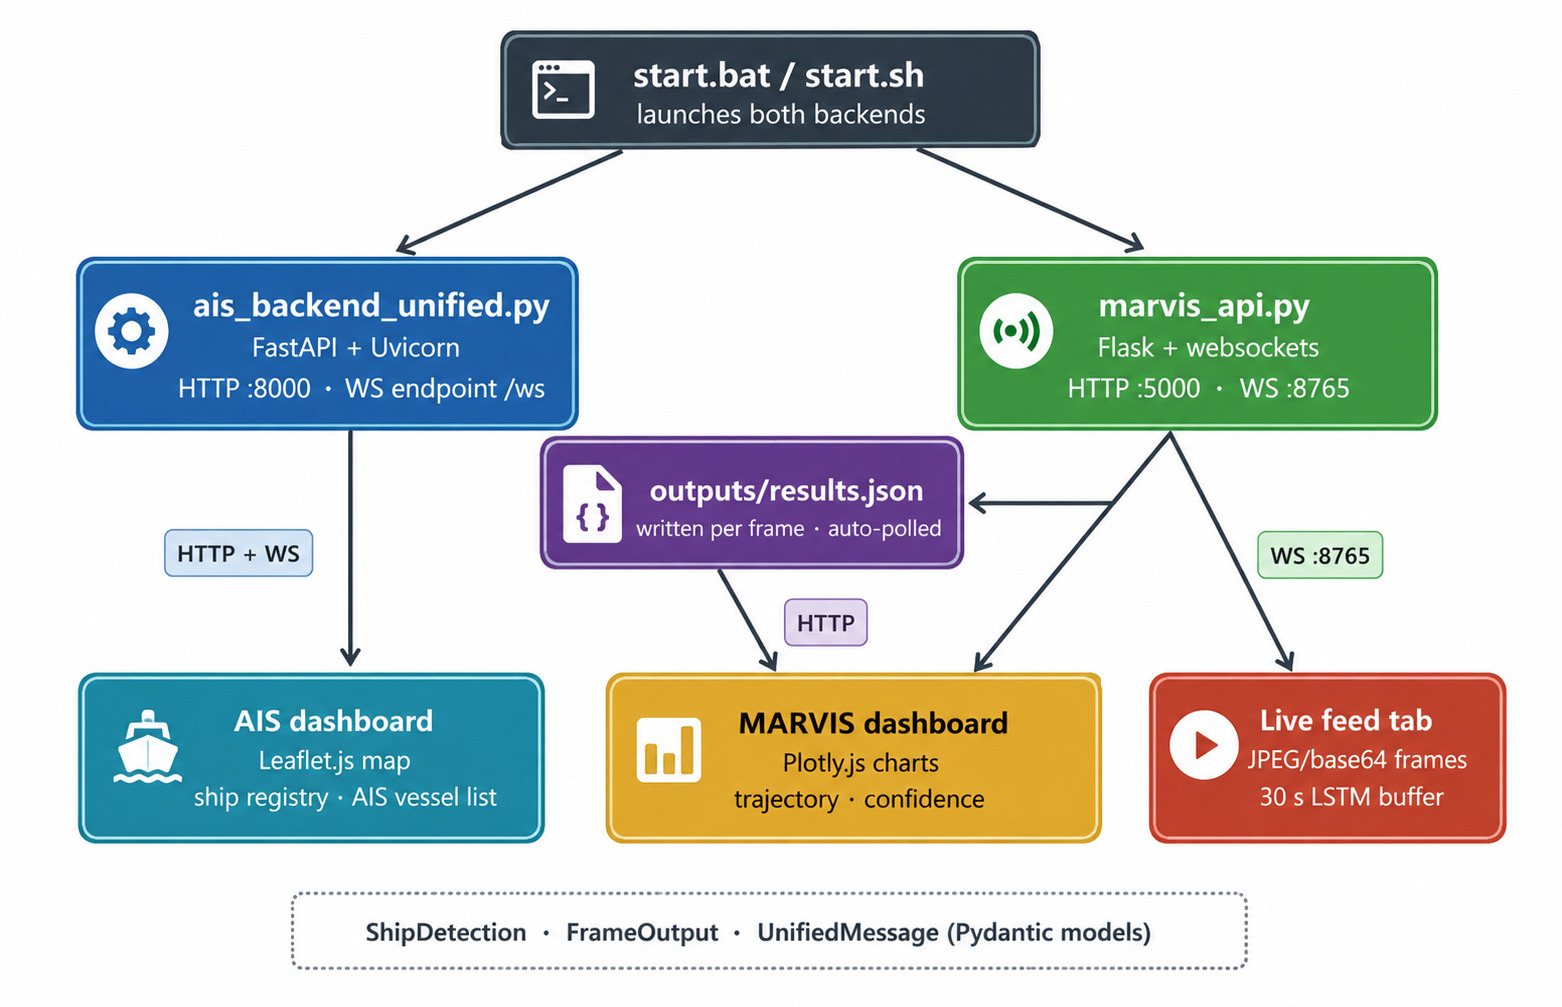
\includegraphics[width=0.95\textwidth]{Chapter4/Figures/dashboard_architecture.jpeg}
\caption{Dashboard Communication and Visualization Architecture}
\label{fig:dashboard}
\end{figure}

\section{Summary}

This chapter provided a detailed examination of the implementation strategies utilized to translate earlier theoretical designs into a fully operational, real-time surveillance infrastructure. The practical realization of the system relied heavily on assembling a robust software stack anchored by Python, \gls{pytorch}, and \gls{opencv}, all operating within a strictly \gls{cuda}-accelerated hardware environment. Taking this approach allowed the architecture to process heavy deep learning workloads continuously, entirely bypassing the frame rate degradation that typically plagues complex visual analysis tasks.

Considerable effort was dedicated to the preparatory phases, involving the construction of a comprehensive dataset segmented into a reliable 70:20:10 split. This careful curation allowed the \gls{yolov8} detection module to be effectively fine-tuned and securely bound to the \gls{deepocsort} tracking algorithm, utilizing \gls{osnet} visual embeddings to maintain identity continuity across frames. Furthermore, the implementation addressed the inherent difficulty of merging distinct sensor modalities. By extracting frame-to-frame motion metrics and projecting pixel data into a geographic coordinate space, the pipeline effectively synchronized optical tracking data with authoritative \gls{ais} broadcasts, stabilizing the fused output through the application of a Kalman filter.

The integration of the stacked \gls{lstm} neural network formed the final analytical tier, tasked with analyzing historical ship movements to output highly reliable trajectory forecasts. The inclusion of a kinematic regression fallback for tracking immature targets, combined with a geographical land-mask filter, fortified the logic against common predictive errors. All computed data streams were successfully routed into dual visualization interfaces, offering both direct video overlays and interactive cartographic mapping. The successful integration of these diverse components results in a unified, end-to-end maritime tracking framework. The operational efficacy and quantitative performance of this complete system will be systematically evaluated and discussed in the subsequent chapter.
